\documentclass[aps,prresearch,reprint,floatfix,superscriptaddress,nofootinbib,longbibliography]{revtex4-2}

\usepackage[T1]{fontenc}
\usepackage{amsmath,amssymb,bm}
\usepackage{booktabs}
\usepackage{graphicx}
\usepackage{tikz}
\usepackage{pgfplots}
\usepackage[hidelinks]{hyperref}
\pgfplotsset{compat=1.18}

\newcommand{\Id}{\mathsf I}
\newcommand{\Proj}{\mathsf P}
\newcommand{\Col}{\operatorname{Col}}
\newcommand{\Null}{\operatorname{Null}}
\newcommand{\rank}{\operatorname{rank}}
\newcommand{\Iprof}{\mathcal I_{\beta}^{\rm prof}}
\newcommand{\Iprior}{\mathcal I_{\beta}(\Lambda)}
\newcommand{\RQIR}{\mathrm{RQIR}}

\begin{document}

\title{Relativity--Quantum Interface Reconstruction II:\\
Statistical Identifiability, Nuisance Geometry, and Detectability in Detector-Facing Likelihoods}

\author{Aleksey Buyanov}
\email{pppuu7@gmail.com}
\thanks{ORCID: \href{https://orcid.org/0009-0001-2621-9305}{0009-0001-2621-9305}}
\affiliation{Independent Researcher, Moscow, Russia}
\date{9 September 2026}

\begin{abstract}
Relativity--Quantum Interface Reconstruction (RQIR) separates exact source-side distinguishability from the statistical question of whether a surviving interface direction can be inferred after nuisance freedoms, detector covariance, and finite information are included. We formulate this second layer for local detector-facing Gaussian likelihoods. After covariance whitening, the target score is a vector $\bm s$ and the nuisance scores form a matrix $J$. For unconstrained nuisance parameters, the profiled Fisher information is the squared distance of $\bm s$ from $\Col(J)$ and is equivalently a generalized Schur complement. With independent nuisance information of precision $\Lambda\succeq0$, we derive the variational identity
$\mathcal I_\beta(\Lambda)=\min_{\bm a}\{\|\bm s-J\bm a\|^2+\bm a^T\Lambda\bm a\}$.
It makes nuisance-coordinate invariance and monotonic recovery under stronger calibration information explicit, while also distinguishing data-only structural identifiability from prior-assisted precision. Exact score alignment is not cured by exposure alone. Conversely, a two-band response with a relative-tilt nuisance self-calibrates with
$\mathcal I_{\beta\mid t}=4g_2^2g_4^2/(g_2^2+g_4^2)$.
We freeze these statements in the seven-test RQIR-STAT-001 regression certificate and independently stress-test the implementation in 10,000 randomized trials, including rank-deficient nuisance matrices and correlated covariance: no invariant violation is observed at the declared numerical tolerances. A minimal cutoff counterexample further shows that deleting a weak but exactly collinear nuisance direction can manufacture a unit Fisher signal from a truly degenerate problem. The result is a calibration-aware statistical layer connecting the exact quotient geometry of RQIR I to resource conversion in RQIR III without conflating algebraic survival, local identifiability, prior-assisted inference, and practical detectability.
\end{abstract}

\maketitle

\section{Introduction}
\label{sec:intro}

An operational signal can survive an exact calibration and still fail as an inferential target. The reason is that three logically distinct questions intervene between a source-side separation and a finite experiment:
\begin{equation}
\begin{aligned}
\text{exact separation}&\;\not\Rightarrow\;\text{statistical identifiability}\\
&\;\not\Rightarrow\;\text{practical detectability}.
\end{aligned}
\label{eq:staging}
\end{equation}
RQIR I formalizes the first layer as a finite calibration quotient on physically admissible source-state perturbations. In its simplest form, a calibration map $A$ can leave a physical null direction $n$ for which a designated response functional $c$ is nonzero,
\begin{equation}
 A n=0,\qquad c(n)\neq0,
\label{eq:paper1bridge}
\end{equation}
so calibration-equivalent positive source states can remain response-distinct \cite{RQIRI}. Equation~\eqref{eq:paper1bridge} is exact. It does not establish that a noisy detector can infer the amplitude of that direction after source, apparatus, calibration, and detector nuisances are introduced.

This distinction is familiar in statistical identification theory. Under regularity conditions, local identifiability is tied to the information matrix \cite{Fisher1922,Rao1945,Rothenberg1971}; nuisance parameters motivate profile or orthogonalized likelihood constructions \cite{CoxReid1987,Cowan2011}. Geometric treatments of nonlinear least squares emphasize that parameter directions are represented by tangent vectors in prediction space \cite{Transtrum2011}. Modern identifiability literature also stresses that structural and practical identifiability are not interchangeable and that Fisher diagnostics alone should not be overinterpreted away from their local regime \cite{Wieland2021,Heinrich2025}. The RQIR problem adds a specific ordering constraint: the likelihood analysis must begin only after the exact source/calibration quotient and detector-facing response map have been declared.

The purpose of this paper is therefore not to invent Fisher information or profile likelihood. It is to close the RQIR statistical layer by binding five ingredients into one auditable framework: (i) the calibration-aware interface inherited from Paper I; (ii) covariance-whitened nuisance geometry; (iii) independent preparation/calibration information treated separately from data-only identifiability; (iv) exact obstruction and self-calibration examples relevant to the retained RQIR detector fronts; and (v) deterministic and property-based regressions designed to catch coordinate, rank-cutoff, and covariance errors before physical resource claims are made.

The main contributions are:
\begin{enumerate}
\item a projection/Schur representation of local nuisance-profiled information, including rank-deficient nuisance score matrices through the Moore--Penrose pseudoinverse \cite{Penrose1955};
\item an exact variational representation with positive-semidefinite nuisance precision, yielding coordinate invariance and calibration-information monotonicity;
\item a clean separation between data-only structural local identifiability and prior-assisted precision;
\item an exposure no-go for exact score alignment and an analytic two-band self-calibration law;
\item a shared-versus-branch-specific nuisance inequality;
\item a seven-test deterministic reference certificate plus a 10,000-trial independent numerical stress audit;
\item an explicit numerical counterexample showing how an arbitrary inverse cutoff can turn exact degeneracy into a false detection.
\end{enumerate}

We do not convert Fisher information into apparatus-specific shot counts, power spectral densities, coherence times, wall-clock times, or technological readiness. That conversion is the subject of RQIR III. We also do not claim global nonlinear identifiability from a local Fisher criterion.

\section{Interface inherited from RQIR I}
\label{sec:interface}

RQIR I orders the inference chain upstream of the likelihood. Schematically, a physical source perturbation is first reduced by exact preparation constraints, then identified modulo a declared finite calibration map, then propagated through a specified detector-facing response. Only after those operations is a statistical data model assigned \cite{RQIRI}. The present paper takes the resulting local detector-facing mean response as its input.

Parameterize the Paper-I physical direction by a local source displacement $\delta q=\beta n$. If $\mathcal R$ denotes the declared detector-facing response map, its local science derivative is
\begin{equation}
 \bm t = D\mathcal R[n]=\partial_\beta\bm\mu.
\label{eq:detectorpush}
\end{equation}
If $D\mathcal R[n]=0$, the direction is erased by the chosen detector transfer before any statistical profiling occurs; this is a detector-map failure, not a nuisance degeneracy. The statistical analysis below begins only after a nonzero or explicitly audited detector derivative has been declared.

Let $\bm d\in\mathbb R^n$ denote a detector-level summary for a fixed experimental configuration. Near an audit point $(\beta_0,\bm\eta_0)$, write
\begin{equation}
 \bm\mu(\beta,\bm\eta)
 =\bm\mu_0
 +(\beta-\beta_0)\,\bm t
 +K(\bm\eta-\bm\eta_0)
 +O(\|\delta\bm\theta\|^2),
\label{eq:localmean}
\end{equation}
where $\beta$ is the target amplitude, $\bm\eta\in\mathbb R^m$ is a nuisance vector, $\bm t=\partial_\beta\bm\mu$, and the columns of $K$ are nuisance derivatives. The covariance at the audit point is $C\succ0$. The local Gaussian reference likelihood is
\begin{equation}
 p(\bm d\mid\beta,\bm\eta)
 \propto |C|^{-1/2}
 \exp\!\left[-\frac12(\bm d-\bm\mu)^T C^{-1}(\bm d-\bm\mu)\right].
\label{eq:gaussian}
\end{equation}
We initially treat $C$ as parameter independent at the audit point. Parameter-dependent covariance contributes the standard additional covariance-derivative Fisher terms and lies outside the frozen RQIR-STAT-001 reference certificate.

Choose any symmetric whitening matrix $W_C=C^{-1/2}$ and define
\begin{equation}
 \bm s=W_C\bm t,\qquad J=W_C K.
\label{eq:whiten}
\end{equation}
Whitening is a coordinate change in data space, not a physical approximation. In these coordinates the local covariance metric is Euclidean.

\section{Unconstrained nuisance geometry}
\label{sec:geometry}

For $\Lambda=0$, the Fisher blocks of the linearized mean model are
\begin{equation}
F=\begin{pmatrix}
\bm s^T\bm s & \bm s^T J\\
J^T\bm s & J^T J
\end{pmatrix}.
\label{eq:fisherblock}
\end{equation}
Let
\begin{equation}
 \Proj_J=J(J^T J)^+J^T=J J^+
\label{eq:projector}
\end{equation}
be the orthogonal projector onto $\Col(J)$.

\paragraph*{Proposition 1 (projection--Schur equivalence).}
For the local Gaussian mean model, including a rank-deficient nuisance score matrix,
\begin{align}
 \Iprof
 &=\| (\Id-\Proj_J)\bm s\|_2^2
\label{eq:projfisher}\\
 &=\bm s^T\bm s-\bm s^T J(J^T J)^+J^T\bm s.
\label{eq:schur}
\end{align}

\emph{Proof.} Equation~\eqref{eq:projector} is the orthogonal projector onto $\Col(J)$. Therefore $\Id-\Proj_J$ is symmetric and idempotent, so its quadratic form is the squared residual norm. Expanding gives Eq.~\eqref{eq:schur}. The pseudoinverse makes the expression independent of redundant nuisance columns. \hfill$\square$

\paragraph*{Proposition 2 (first-order local identifiability).}
In the data-only local model, the target score is distinguishable to first order from nuisance motion if and only if
\begin{equation}
 \Iprof>0
 \quad\Longleftrightarrow\quad
 \bm s\notin\Col(J).
\label{eq:identcrit}
\end{equation}

\emph{Proof.} The left side of Eq.~\eqref{eq:projfisher} is a squared norm. It vanishes exactly when $\bm s=\Proj_J\bm s$, i.e. when $\bm s$ belongs to the nuisance span. \hfill$\square$

The qualifier ``first-order local'' is essential. Curvature of a nonlinear model manifold can break a tangent degeneracy at higher order, while disconnected parameter values can remain globally aliased even when the local tangent is nondegenerate. Our usage is therefore compatible with the distinction between local structural and practical identifiability emphasized in the broader literature \cite{Rothenberg1971,Wieland2021,Heinrich2025}.

A useful dimensionless diagnostic is the retained fraction
\begin{equation}
 \rho_\beta=\frac{\Iprof}{\bm s^T\bm s},\qquad 0\le\rho_\beta\le1,
\label{eq:retention}
\end{equation}
provided the raw target Fisher is nonzero. This ratio measures local information lost to nuisance profiling, not experimental feasibility.

\paragraph*{Proposition 3 (nuisance enrichment).}
If $\mathcal N_1\subseteq\mathcal N_2$ are nested nuisance score spans, then
\begin{equation}
 \mathcal I_\beta(\mathcal N_2)\le \mathcal I_\beta(\mathcal N_1).
\label{eq:nuisancemono}
\end{equation}

\emph{Proof.} Equation~\eqref{eq:projfisher} is the squared Euclidean distance of $\bm s$ from the nuisance subspace. The distance to a larger subspace cannot be greater. \hfill$\square$

This elementary fact is a powerful regression test: adding an unconstrained nuisance direction cannot increase data-only profiled information unless some other element of the experiment or prior model also changes.


\section{Independent nuisance information and the variational form}
\label{sec:prior}

Preparation measurements, calibration data, or external control information can constrain nuisance coefficients. Let $\Lambda\succeq0$ denote the corresponding independent local precision matrix. The combined Fisher block is
\begin{equation}
F_\Lambda=\begin{pmatrix}
\bm s^T\bm s & \bm s^T J\\
J^T\bm s & J^T J+\Lambda
\end{pmatrix},
\end{equation}
and the profiled target information is
\begin{equation}
 \Iprior=\bm s^T\bm s-
 \bm s^T J(J^TJ+\Lambda)^+J^T\bm s.
\label{eq:priorfisher}
\end{equation}

\paragraph*{Proposition 4 (variational profiling identity).}
For $\Lambda\succeq0$,
\begin{equation}
 \boxed{\displaystyle
 \Iprior=\min_{\bm a\in\mathbb R^m}
 \left[\|\bm s-J\bm a\|_2^2+\bm a^T\Lambda\bm a\right].}
\label{eq:variational}
\end{equation}

\emph{Proof.} Expand the objective as
\begin{equation}
 \bm s^T\bm s-2\bm a^TJ^T\bm s
 +\bm a^T(J^TJ+\Lambda)\bm a.
\end{equation}
For every $z\in\Null(J^TJ+\Lambda)$, positivity of both terms implies $Jz=0$ and $\Lambda^{1/2}z=0$, hence $z^TJ^T\bm s=0$. Thus $J^T\bm s$ belongs to the range of $J^TJ+\Lambda$ and the minimum is attained by the pseudoinverse solution. Substitution gives Eq.~\eqref{eq:priorfisher}. \hfill$\square$

Two corollaries are immediate.

\paragraph*{Corollary 4.1 (nuisance-coordinate invariance).}
For any invertible nuisance transformation $\bm a=M\bm\phi$,
\begin{equation}
 J_\phi=JM,\qquad \Lambda_\phi=M^T\Lambda M,
\end{equation}
and $\mathcal I_\beta$ is unchanged. This follows because Eq.~\eqref{eq:variational} is the same minimization written in bijectively related coordinates.

\paragraph*{Corollary 4.2 (calibration-information monotonicity).}
If $\Lambda_2-\Lambda_1\succeq0$, then
\begin{equation}
 \mathcal I_\beta(\Lambda_2)\ge\mathcal I_\beta(\Lambda_1).
\label{eq:priormono}
\end{equation}
For every trial nuisance coefficient, the objective in Eq.~\eqref{eq:variational} can only increase when a positive-semidefinite penalty is added; therefore its minimum cannot decrease.

The language here requires care. If $\bm s\in\Col(J)$, the target is not structurally identifiable from the detector data alone at first order, even if $\mathcal I_\beta(\Lambda)>0$ after external nuisance information is added. The latter is \emph{prior-assisted or calibration-assisted precision}, not data-only identification. This distinction prevents an external constraint from being misreported as information created by the science channel.

\subsection{Exact amplitude obstruction and prior rescue}

The minimal RQIR reference model takes
\begin{equation}
 \bm s_0=(1,0)^T,\qquad J=\bm s_0.
\end{equation}
The science and nuisance scores are exactly aligned, so $\mathcal I_\beta(0)=0$. If an independent preparation measurement contributes scalar precision $C_a$, Eq.~\eqref{eq:priorfisher} gives
\begin{equation}
 \boxed{\displaystyle
 \mathcal I_\beta(C_a)=\frac{C_a}{1+C_a}.}
\label{eq:priorrescue}
\end{equation}
The RQIR-STAT-001 certificate checks $C_a=1,4,9,19,99$, giving $0.5,0.8,0.9,0.95,0.99$, respectively.

\begin{figure}[t]
\centering
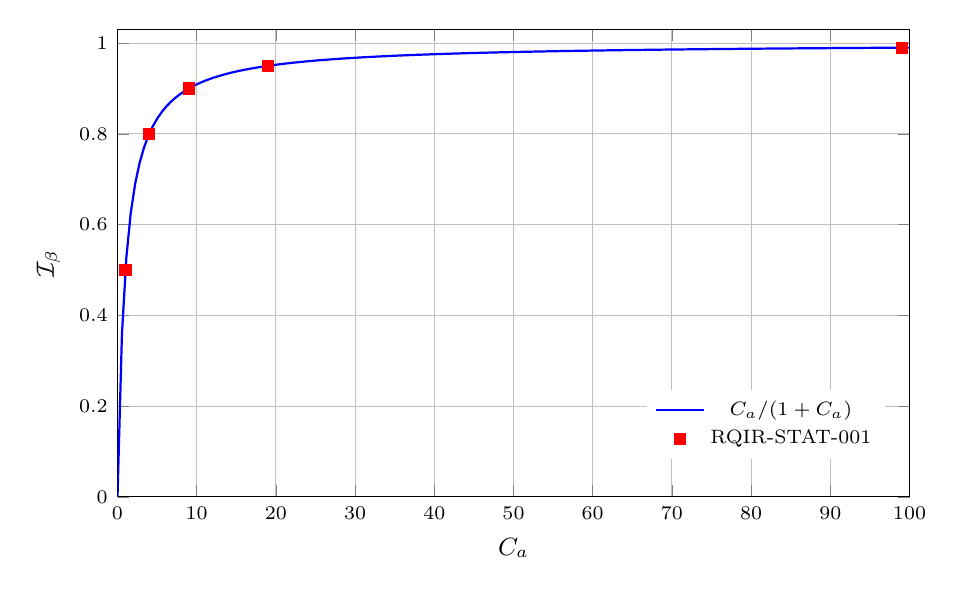
\begin{tikzpicture}
\begin{axis}[
 width=0.96\columnwidth,height=0.62\columnwidth,
 xlabel={$C_a$},ylabel={$\mathcal I_\beta$},
 xmin=0,xmax=100,ymin=0,ymax=1.03,
 grid=major,legend style={font=\scriptsize,draw=none,at={(0.97,0.08)},anchor=south east},
 tick label style={font=\scriptsize},label style={font=\small}]
\addplot[blue,thick,domain=0:100,samples=180] {x/(1+x)};
\addlegendentry{$C_a/(1+C_a)$}
\addplot[only marks,mark=square*,red] coordinates {(1,0.5) (4,0.8) (9,0.9) (19,0.95) (99,0.99)};
\addlegendentry{RQIR-STAT-001}
\end{axis}
\end{tikzpicture}

\caption{Calibration-assisted recovery for the exactly aligned amplitude model, Eq.~\eqref{eq:priorrescue}. The curve approaches the unit raw Fisher but never changes the fact that the detector data alone have zero first-order information at $C_a=0$. Markers are deterministic RQIR-STAT-001 points. Plotting code was AI-assisted; values were checked by a separate deterministic audit script against the analytic formula.}
\label{fig:priorrescue}
\end{figure}


\section{Exposure, self-calibration, and finite-data staging}
\label{sec:detectability}

\subsection{Exposure cannot cure exact alignment}

Let exposure $E$ scale both science and unconstrained nuisance scores as
\begin{equation}
 \bm s_E=\sqrt E\,\bm s,
 \qquad J_E=\sqrt E\,J.
\end{equation}
If $\bm s=J\bm a$ for some $\bm a$, then $\bm s_E=J_E\bm a$ for every $E>0$, so Proposition 2 gives
\begin{equation}
 \mathcal I_\beta(E)=0\qquad\forall E>0.
\label{eq:exposureno}
\end{equation}
RQIR-STAT-001 checks this explicitly from $E=1$ through $10^6$. ``More data'' therefore does not resolve an exact unconstrained nuisance degeneracy; a new response direction or independent nuisance information is required.

When $\mathcal I_\beta>0$ and independent observations add Fisher information, the local Cram\'er--Rao scaling is
\begin{equation}
 \sigma_\beta\gtrsim [N\mathcal I_\beta]^{-1/2}.
\label{eq:cramerrao}
\end{equation}
Equation~\eqref{eq:cramerrao} is only a staging relation. Translating $N$ or $\mathcal I_\beta$ into physical apparatus resources belongs to Paper III.

\subsection{Two-band self-calibration}

A complementary example shows how response diversity can break a nuisance degeneracy without an external prior. Let the whitened science score and a relative spectral-tilt nuisance be
\begin{equation}
 \bm g=(g_2,g_4)^T,
 \qquad
 \bm t=(g_2,-g_4)^T.
\end{equation}
Profiling the tilt gives
\begin{align}
 \mathcal I_{\beta\mid t}
 &=\bm g^T\bm g-
 \frac{(\bm g^T\bm t)^2}{\bm t^T\bm t}\\
 &=\boxed{\displaystyle\frac{4g_2^2g_4^2}{g_2^2+g_4^2}}.
\label{eq:twoband}
\end{align}
For $(g_2,g_4)=(0.3,0.7)$, the raw Fisher is $0.58$ and the profiled value is
\begin{equation}
 \mathcal I_{\beta\mid t}=0.3041379310344828,
\end{equation}
so the retained fraction is $\rho_\beta=0.5243757431629014$.

\begin{figure}[t]
\centering
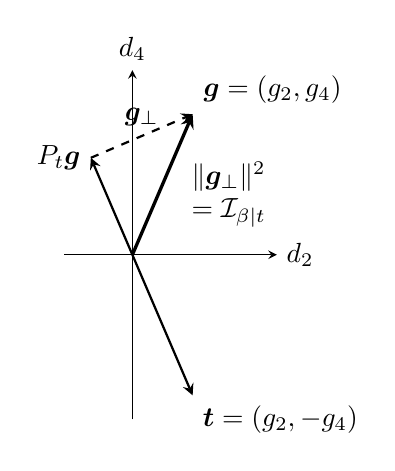
\begin{tikzpicture}[>=stealth,scale=2.55]
\draw[->] (-0.34,0) -- (0.72,0) node[right] {$d_2$};
\draw[->] (0,-0.82) -- (0,0.92) node[above] {$d_4$};
\coordinate (O) at (0,0);
\coordinate (G) at (0.30,0.70);
\coordinate (T) at (0.30,-0.70);
\coordinate (P) at (-0.2069,0.4828);
\draw[->,very thick] (O) -- (G) node[above right] {$\bm g=(g_2,g_4)$};
\draw[->,thick] (O) -- (T) node[below right] {$\bm t=(g_2,-g_4)$};
\draw[->,thick] (O) -- (P) node[left] {$P_t\bm g$};
\draw[->,thick,dashed] (P) -- (G) node[midway,above] {$\bm g_\perp$};
\node[align=left] at (0.48,0.30) {$\|\bm g_\perp\|^2$\\$=\mathcal I_{\beta\mid t}$};
\end{tikzpicture}

\caption{Whitened nuisance geometry for the two-band example. The target vector $\bm g$ is decomposed into a projection along the tilt nuisance and an orthogonal residual $\bm g_\perp$; the squared residual norm is the profiled Fisher information. The schematic geometry was AI-assisted and verified against Eq.~\eqref{eq:twoband}.}
\label{fig:geometry}
\end{figure}

Writing $r=g_4/g_2$, the retention becomes
\begin{equation}
 \rho_\beta(r)=\frac{4r^2}{(1+r^2)^2}.
\label{eq:rhoratio}
\end{equation}
It peaks at unity for balanced magnitudes $r=1$ and tends to zero when either band dominates. Thus ``adding a channel'' is not, by itself, the relevant statement; the new channel must rotate the science response relative to the nuisance span.

\begin{figure}[t]
\centering
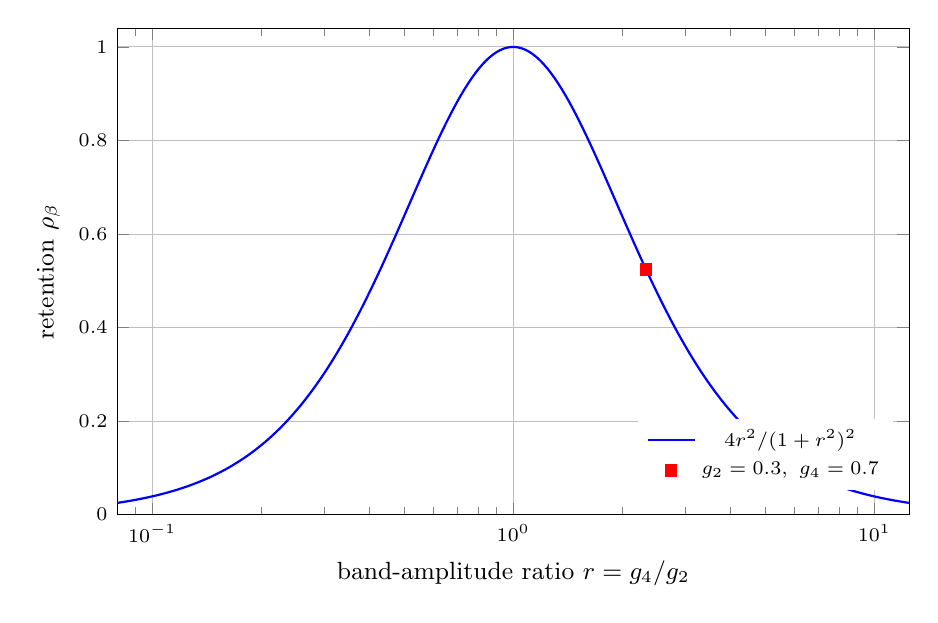
\begin{tikzpicture}
\begin{axis}[
 width=0.96\columnwidth,height=0.64\columnwidth,
 xmode=log,xmin=0.08,xmax=12.5,ymin=0,ymax=1.04,
 xlabel={band-amplitude ratio $r=g_4/g_2$},ylabel={retention $\rho_\beta$},
 grid=major,legend style={font=\scriptsize,draw=none,at={(0.98,0.05)},anchor=south east},
 tick label style={font=\scriptsize},label style={font=\small}]
\addplot[blue,thick,domain=0.08:12.5,samples=220] {4*x^2/(1+x^2)^2};
\addlegendentry{$4r^2/(1+r^2)^2$}
\addplot[only marks,mark=square*,red] coordinates {(2.3333333333,0.5243757431629014)};
\addlegendentry{$g_2=0.3,\ g_4=0.7$}
\end{axis}
\end{tikzpicture}

\caption{Two-band information retention, Eq.~\eqref{eq:rhoratio}. Balanced response gives complete local separation from the antisymmetric tilt nuisance, whereas strong band imbalance restores an approximate degeneracy. The marked RQIR-STAT-001 point retains about $52.44\%$ of the raw local Fisher information. Plotting code was AI-assisted and checked against archived curve data.}
\label{fig:retention}
\end{figure}

\subsection{A synthetic information-retention map}

To visualize the distinction between exact structural alignment, weak misalignment, and prior assistance, consider the normalized analytic family
\begin{equation}
 \bm s=(1,0)^T,\qquad
 \bm j=(1,\delta)^T,
\end{equation}
with scalar prior precision $\lambda\ge0$. Equation~\eqref{eq:priorfisher} gives
\begin{equation}
 \rho_\beta(\delta,\lambda)
 =\mathcal I_\beta(\delta,\lambda)
 =\frac{\delta^2+\lambda}{1+\delta^2+\lambda}.
\label{eq:map}
\end{equation}
The point $(0,0)$ is structurally degenerate; any nonzero $\delta$ creates data-only local identifiability, but the information can remain arbitrarily small. Nonzero $\lambda$ can instead supply prior-assisted precision even at $\delta=0$.

\begin{figure}[t]
\centering
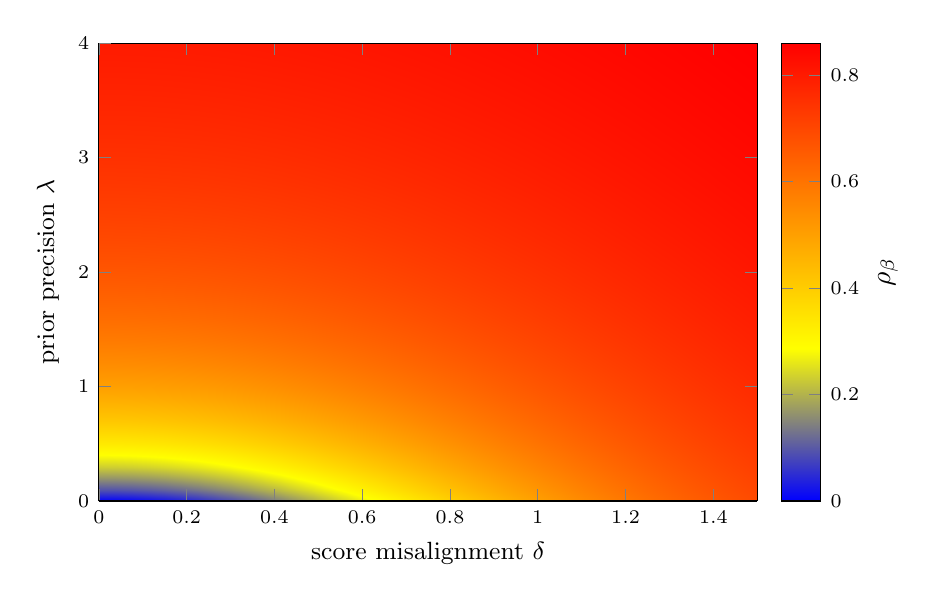
\begin{tikzpicture}
\begin{axis}[
 width=0.82\columnwidth,height=0.61\columnwidth,
 view={0}{90},xmin=0,xmax=1.5,ymin=0,ymax=4,
 xlabel={score misalignment $\delta$},ylabel={prior precision $\lambda$},
 colorbar,colorbar style={ylabel={$\rho_\beta$},yticklabel style={font=\scriptsize}},
 point meta min=0,point meta max=0.86,
 tick label style={font=\scriptsize},label style={font=\small}]
\addplot3[surf,shader=interp,domain=0:1.5,domain y=0:4,samples=41]
 {(x^2+y)/(1+x^2+y)};
\end{axis}
\end{tikzpicture}

\caption{Synthetic analytic information-retention map for Eq.~\eqref{eq:map}. The horizontal axis rotates the nuisance score away from exact alignment; the vertical axis adds independent nuisance precision. This is an identifiability diagnostic, not a physical reach forecast. Plotting code was AI-assisted and checked against archived grid data generated directly from Eq.~\eqref{eq:map}.}
\label{fig:map}
\end{figure}

\section{Shared and branch-specific nuisances}
\label{sec:branches}

Multiple detector branches or data subsets can share physical nuisance coefficients. The distinction between a genuinely shared nuisance and independent branchwise copies changes the nuisance subspace.

For independent data blocks $b=1,\ldots,B$, stack target scores and shared-nuisance matrices,
\begin{equation}
 \bm s=\begin{bmatrix}\bm s_1\\ \vdots\\ \bm s_B\end{bmatrix},
 \qquad
 J_{\rm sh}=\begin{bmatrix}J_1\\ \vdots\\ J_B\end{bmatrix}.
\end{equation}
If the same nuisance coefficient is instead allowed to vary independently in each branch, the nuisance matrix is
\begin{equation}
 J_{\rm sep}=\operatorname{diag}(J_1,\ldots,J_B).
\end{equation}

\paragraph*{Proposition 5 (shared-nuisance information bound).}
When the only difference is replacing one genuinely shared nuisance vector by unconstrained branch-specific copies,
\begin{equation}
 \mathcal I_{\rm shared}\ge \mathcal I_{\rm separate}.
\label{eq:sharedbound}
\end{equation}

\emph{Proof.} Every stacked displacement generated by a shared coefficient can also be generated by choosing equal branchwise copies, so
$\Col(J_{\rm sh})\subseteq\Col(J_{\rm sep})$ in the stacked data space. Proposition 3 then gives Eq.~\eqref{eq:sharedbound}. \hfill$\square$

The result is practically important: summing independently profiled branch Fishers is generally more conservative than a joint fit when the nuisance is truly shared. Conversely, imposing a shared nuisance without a physical justification can overstate information. The physical sharing structure must be declared before profiling.

\section{Correlated covariance and whitening invariance}
\label{sec:covariance}

For an unwhitened target derivative $\bm t$, nuisance matrix $K$, and positive-definite covariance $C$, the data-only profile is
\begin{equation}
 \mathcal I_\beta=
 \bm t^T C^{-1}\bm t
 -\bm t^T C^{-1}K
 (K^TC^{-1}K)^+
 K^TC^{-1}\bm t.
\label{eq:fullcov}
\end{equation}
Exact whitening by $C^{-1/2}$ maps Eq.~\eqref{eq:fullcov} to Eq.~\eqref{eq:schur}. Thus the geometry does not assume diagonal detector noise; it assumes only that the covariance used in the local reference likelihood is declared and positive definite on the retained data space.

As an additional submission-level regression beyond the historical seven-test certificate, we generated a deterministic correlated covariance with seed 20260908, dimension six, nuisance dimension two, and $\kappa(C)=21.4642$. Direct evaluation of Eq.~\eqref{eq:fullcov} gives $6.8036503258133445$; symmetric whitening gives $6.803650325813313$, an absolute difference $3.11\times10^{-14}$. The 10,000-trial stress audit described below found a maximum whitening discrepancy $5.97\times10^{-13}$ and no failures at tolerance $10^{-8}$.

\section{RQIR-STAT-001 deterministic reference certificate}
\label{sec:certificate}

The retained Paper-II science scope is frozen by the source-agnostic RQIR-STAT-001 reference-likelihood certificate. Its purpose is not to substitute for an apparatus model; it enforces algebraic invariants that any later detector likelihood must satisfy before resource calculations are credited. Table~\ref{tab:certificate} records an independent rerun against the current repository implementation.

\begin{table*}[t]
\caption{Submission rerun of the seven deterministic RQIR-STAT-001 regressions. All numbers were recomputed from the current certificate script with fixed seed 20260830. ``PASS'' means the stated analytic or invariant relation was satisfied at the certificate tolerance.}
\label{tab:certificate}
\begin{ruledtabular}
\begin{tabular}{p{0.20\textwidth}p{0.46\textwidth}p{0.23\textwidth}c}
Test & Invariant or expected result & Independent rerun & Status\\
\hline
A. Projection--Schur & $\mathcal I_\beta=\|(I-P_J)s\|^2$ & $1.1749239290799913$ vs. $1.1749239290799873$; $|\Delta|=4.00\times10^{-15}$ & PASS\\
B. Nuisance coordinates & $J\to JM$, $\Lambda\to M^T\Lambda M$ leaves $\mathcal I_\beta$ invariant & $1.8405965236299755$ vs. $1.8405965236299728$; $|\Delta|=2.66\times10^{-15}$ & PASS\\
C. Stronger nuisance information & $\Lambda_2-\Lambda_1\succeq0\Rightarrow \mathcal I_2\ge\mathcal I_1$ & $1.8405965236299755\to2.6370745801113067$ & PASS\\
D. Exact amplitude obstruction & $\mathcal I(C_a)=C_a/(1+C_a)$ & $C_a=9\to0.9$; all six stored values exact to tolerance & PASS\\
E. Exposure obstruction & exact alignment remains zero for any common exposure scaling & $E=1,2,10,100,10^6\to0$ & PASS\\
F. Two-band tilt & $4g_2^2g_4^2/(g_2^2+g_4^2)$ & $0.3041379310344828$ for $(0.3,0.7)$ & PASS\\
G. Rank-cutoff counterexample & true profile $\simeq0$; threshold deletion can return $1$ & $1.11\times10^{-16}$ vs. $1$ & PASS\\
\end{tabular}
\end{ruledtabular}
\end{table*}

These tests close several distinct failure modes. Tests A--C protect algebraic and coordinate consistency. Tests D and E distinguish an exact physical nuisance obstruction from low exposure. Test F demonstrates self-calibration by response diversity. Test G protects weak but physically aligned nuisance directions from arbitrary numerical deletion.

\section{Independent randomized stress audit}
\label{sec:stress}

A deterministic certificate can accidentally validate only its chosen examples. We therefore performed an independent property-based audit with seed 20260908 over 10,000 randomized problems. Data dimensions ranged from 4 to 11 and nuisance dimensions up to 4; every fifth trial was made intentionally rank deficient by replacing one nuisance column with an exact linear combination of the others. Separate random trials tested correlated positive-definite covariances.

The audit checked six properties: projection--Schur equality, nuisance-coordinate invariance with transformed priors, monotonicity under an added positive-semidefinite nuisance precision, exact-alignment collapse, the shared-nuisance bound, and full-covariance/whitening equivalence. No violation occurred at the declared tolerances. Table~\ref{tab:stress} reports the worst observed numerical discrepancies.

\begin{table}[t]
\caption{Independent 10,000-trial submission stress audit. The tolerances are deliberately looser than machine precision to accommodate ill-conditioned random coordinate changes; no trial exceeded them.}
\label{tab:stress}
\begin{ruledtabular}
\begin{tabular}{p{0.52\columnwidth}r}
Diagnostic & Worst or minimum value\\
\hline
max $|\mathcal I_{\rm Schur}-\mathcal I_{\rm proj}|$ & $1.31\times10^{-13}$\\
max nuisance-coordinate discrepancy & $1.02\times10^{-11}$\\
min stronger-prior gain & $2.13\times10^{-11}$\\
min $(\mathcal I_{\rm shared}-\mathcal I_{\rm separate})$ & $2.53\times10^{-7}$\\
max covariance-whitening discrepancy & $5.97\times10^{-13}$\\
violations in six property classes & $0$\\
\end{tabular}
\end{ruledtabular}
\end{table}

The randomized audit is a numerical robustness check, not a replacement for the analytic propositions. Its purpose is to detect implementation errors in rank-deficient, reparameterized, and correlated-covariance cases that are easy to miss with a single fixture.

The standalone submission-audit script used for this section was generated and debugged with substantive assistance from OpenAI ChatGPT (GPT-5.6 Sol). The executable outputs reported here were accepted only after comparison with the frozen deterministic certificate, direct analytic identities, and independent property checks with fixed seeds; the AI system was not used as a numerical authority.

\section{Numerical rank discipline: a minimal false-detection counterexample}
\label{sec:rank}

Pseudoinverse tolerances can change the physics if they are used to delete weak nuisance directions by norm alone. Consider
\begin{equation}
 \bm s=(1,0)^T,
 \qquad
 \bm j=(\epsilon,0)^T,
 \qquad \epsilon=10^{-8}.
\label{eq:cutoffcase}
\end{equation}
The nuisance norm is tiny, but its span is exactly the science direction. Exact geometric profiling therefore gives zero information, numerically $1.11\times10^{-16}$ in the stored floating-point calculation.

A bad implementation that discards the nuisance whenever $j^Tj\le\tau$ instead returns
\begin{equation}
 \mathcal I_{\rm bad}=1
\end{equation}
for any $\tau\ge10^{-16}$. In particular, the historical counterexample uses $\tau=10^{-12}$. The apparent ``detection'' is created entirely by a numerical cutoff.

\begin{figure}[t]
\centering
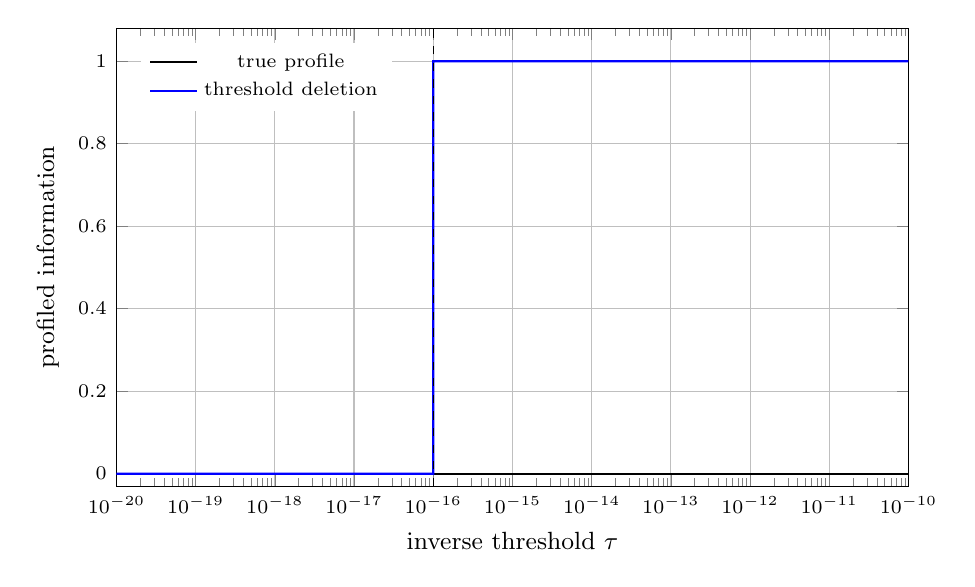
\begin{tikzpicture}
\begin{axis}[
 width=0.96\columnwidth,height=0.61\columnwidth,
 xmode=log,xmin=1e-20,xmax=1e-10,ymin=-0.03,ymax=1.08,
 xlabel={inverse threshold $\tau$},ylabel={profiled information},
 grid=major,legend style={font=\scriptsize,draw=none,at={(0.03,0.97)},anchor=north west},
 tick label style={font=\scriptsize},label style={font=\small}]
\addplot[black,thick] coordinates {(1e-20,0) (1e-10,0)};
\addlegendentry{true profile}
\addplot[blue,thick] coordinates {(1e-20,0) (9.99e-17,0) (1e-16,1) (1e-10,1)};
\addlegendentry{threshold deletion}
\addplot[dashed] coordinates {(1e-16,-0.03) (1e-16,1.08)};
\end{axis}
\end{tikzpicture}

\caption{RQIR-NUM-001 cutoff counterexample. The exact nuisance span is collinear with the science score for every nonzero $\epsilon$, so the true profile remains zero. A threshold-deletion implementation jumps discontinuously to unit information once the inverse cutoff exceeds $\epsilon^2=10^{-16}$. Plotting code was AI-assisted and checked against the analytic branch condition and archived scan data.}
\label{fig:cutoff}
\end{figure}

The methodological rule is therefore stronger than ``choose a small tolerance'': exact hard constraints should be eliminated analytically where possible, and weak physical nuisance directions must not be removed merely because their singular values are small. Numerical regularization must be justified relative to a physical prior, an explicit model reduction, or a demonstrated stability criterion.

\section{Relation to profile likelihood and practical identifiability}
\label{sec:profile}

Fisher information is a local curvature diagnostic. For the linear Gaussian reference model used here, however, the connection to profiling is exact. With whitened residual $\bm r$ and quadratic nuisance precision $\Lambda$, the penalized negative log likelihood is, up to constants,
\begin{equation}
 \ell(\beta,\bm a)
 =\frac12\|\bm r-\beta\bm s-J\bm a\|^2
 +\frac12\bm a^T\Lambda\bm a.
\end{equation}
Profiling over $\bm a$ yields a quadratic function of $\beta$ whose curvature is precisely $\mathcal I_\beta(\Lambda)$ from Eq.~\eqref{eq:variational}. Thus the present Fisher geometry is not an additional approximation \emph{inside the frozen local linear-Gaussian model}.

Outside that local regime, full profile likelihoods can reveal asymmetry, boundaries, curvature, or disconnected solutions that a Fisher matrix misses \cite{CoxReid1987,Wieland2021,Heinrich2025}. Consequently, a future apparatus-specific likelihood should use the present framework as a gate and regression standard, then inspect nonlinear profiles when the actual response model is sufficiently mature. Positive local Fisher is necessary for first-order local inferability in this setting; it is not a universal certificate of global or practical identifiability.

\section{Claims, non-claims, and scope boundary}
\label{sec:scope}

The scientific claims supported here are deliberately narrower than a physical reach forecast.

\begin{table*}[t]
\caption{Interpretation discipline for RQIR II.}
\label{tab:claims}
\begin{ruledtabular}
\begin{tabular}{p{0.27\textwidth}p{0.31\textwidth}p{0.31\textwidth}}
Layer & What can be concluded & What is not implied\\
\hline
Exact Paper-I quotient & a declared calibration leaves a response-sensitive physical direction & finite-noise inference or uniqueness of microscopic gravity\\
Data-only local Fisher & target tangent has a component outside nuisance span & global nonlinear identifiability or practical detectability\\
Prior-assisted profile & combined science+external information constrains $\beta$ locally & detector data alone identify $\beta$\\
Exposure scaling & positive information can accumulate under repeated independent data & exact degeneracy can be cured by more of the same data\\
Two-band self-calibration & response diversity can rotate target away from tilt nuisance & every added channel improves identifiability\\
RQIR-STAT-001 PASS & implementation obeys frozen reference invariants & apparatus readiness, new physics, or a physical resource forecast\\
\end{tabular}
\end{ruledtabular}
\end{table*}

In particular, this paper does not claim evidence that gravity is quantized; it does not claim that the ordered response coordinate isolated in Paper I is transmitted by nature; it does not claim that a Fisher-positive detector front is technologically feasible; and it does not claim that all RQIR branches are identifiable under one nuisance set. Physical source and detector models must declare their own nuisance columns, covariance, shared-parameter structure, and independent calibration information.

\section{Discussion}
\label{sec:discussion}

The main conceptual result of RQIR II is an ordering rule for inference. Paper I can establish an exact response-distinct direction inside a finite calibration equivalence class, but that direction must next pass through the nuisance tangent geometry of the detector likelihood. In whitened space the question is concrete: how much of the science score survives projection onto all allowed nuisance directions? If none survives, exposure alone cannot help. If some survives, its magnitude controls local precision but not yet physical feasibility. If independent preparation information is added, the increase in precision must be labeled as externally assisted rather than attributed to the science data.

The variational form, Eq.~\eqref{eq:variational}, is especially useful because it unifies several audit rules. It makes arbitrary nuisance coordinates irrelevant, proves that genuinely additional independent nuisance information cannot worsen the profiled science information, and provides a stable interpretation even when nuisance columns are redundant. The two-band example then shows the complementary design principle: changing response geometry can create information without an external prior by preventing science and nuisance scores from remaining parallel.

The numerical audit exposes a separate hazard. Statistical identifiability is a statement about subspaces, not nuisance-vector norm. A physically weak nuisance can be exactly aligned with the target, so norm-based threshold deletion changes the model rather than merely stabilizing its inversion. RQIR-NUM-001 turns this point into a minimal regression that can be carried forward to every apparatus-specific implementation.

There are also clear limitations. First, the frozen certificate is synthetic and source-agnostic; it validates likelihood algebra, not any one laboratory architecture. Second, the main theorems are local and first order. Third, the reference covariance is parameter independent at the audit point. Fourth, the current figures are analytic or synthetic diagnostic maps rather than measured reach curves. Fifth, independent calibration information is represented locally by a quadratic precision matrix; non-Gaussian or bounded nuisance constraints require full likelihood treatment. Finally, the present article stops before converting information into physical resources, by design.

These limitations are not unresolved holes in the Paper-II theorem layer; they define the handoff. RQIR III must bind surviving information to shots, spectral densities, coherence, integration time, geometry and control budgets. RQIR IV must then test existing gravity/interface models through a common comparator funnel. Keeping these stages separate prevents a local statistical result from being promoted prematurely into an ontological or technological claim.

\section{Conclusion}
\label{sec:conclusion}

We closed the statistical-identifiability layer of RQIR between exact calibration-aware source separation and physical resource conversion. In a local detector-facing Gaussian likelihood, nuisance profiling has a direct geometry: the data-only Fisher information is the squared distance of the whitened target score from the nuisance tangent span. With independent nuisance information, the exact variational representation
\begin{equation}
 \mathcal I_\beta(\Lambda)=\min_{\bm a}
 \bigl[\|\bm s-J\bm a\|^2+\bm a^T\Lambda\bm a\bigr]
\end{equation}
separates external constraint from science-channel geometry and yields coordinate invariance and monotonicity.

Two exact consequences sharpen the experimental interpretation. Exact score alignment is not repaired by more exposure of the same experiment. Response diversity can instead self-calibrate, as shown by the two-band law $4g_2^2g_4^2/(g_2^2+g_4^2)$. A seven-test deterministic certificate reproduces these results, and an independent 10,000-trial stress audit finds no violation of the analytic invariants under rank deficiency, coordinate changes, shared-versus-separate nuisances, or correlated covariance at the declared tolerances. Conversely, a weak-nuisance cutoff counterexample demonstrates that careless numerical thresholding can create a false unit-information signal from an exactly degenerate problem.

The resulting inference ladder is therefore explicit: exact calibration survival, data-only local identifiability, prior-assisted precision, finite-data sensitivity, and physical resource closure are different statements. RQIR II supplies the statistical gate between the first and the last of these statements.

\begin{acknowledgments}
The numerical audit and manuscript-development workflow made substantive use of OpenAI ChatGPT (GPT-5.6 Sol, accessed September 2026) for algebraic cross-checking, generation and debugging of audit code, numerical stress testing, literature organization, figure-source generation, and manuscript drafting. The tool was directed to preserve explicit claim/non-claim boundaries and to verify generated numerical claims against deterministic repository scripts and separately generated regression calculations. The AI tool is not an author. The author retains full responsibility for the accuracy, interpretation, and integrity of the submitted work.
\end{acknowledgments}

\section*{Data availability}
All code and numerical data used to reproduce the tables and figures in this article are openly available in the Relativity--Quantum Interface Reconstruction repository \cite{RQIRRepo}. The exact audit/data snapshot used for this manuscript is repository commit \texttt{d0f6453721821fcaec4e9e24ea5e68185d90a5a2}, which contains the audit JSON, vector figure sources, and the standalone submission-audit script that regenerates all diagnostic curve/grid CSV files. The deterministic RQIR-STAT-001 seed is 20260830 and the independent 10,000-trial audit seed is 20260908.

\begin{thebibliography}{99}

\bibitem{RQIRI}
A. Buyanov, ``Relativity--Quantum Interface Reconstruction I: Operational Hierarchy, Ordered Stress--Energy Information, and Finite Calibration-Nullspace Discriminants,'' working manuscript v0.6 (8 September 2026).

\bibitem{Fisher1922}
R. A. Fisher, ``On the Mathematical Foundations of Theoretical Statistics,'' Philos. Trans. R. Soc. London A \textbf{222}, 309--368 (1922), doi:10.1098/rsta.1922.0009.

\bibitem{Rao1945}
C. R. Rao, ``Information and the Accuracy Attainable in the Estimation of Statistical Parameters,'' Bull. Calcutta Math. Soc. \textbf{37}, 81--91 (1945).

\bibitem{Rothenberg1971}
T. J. Rothenberg, ``Identification in Parametric Models,'' Econometrica \textbf{39}, 577--591 (1971), doi:10.2307/1913267.

\bibitem{CoxReid1987}
D. R. Cox and N. Reid, ``Parameter Orthogonality and Approximate Conditional Inference,'' J. R. Stat. Soc. B \textbf{49}, 1--18 (1987), doi:10.1111/j.2517-6161.1987.tb01422.x.

\bibitem{Cowan2011}
G. Cowan, K. Cranmer, E. Gross, and O. Vitells, ``Asymptotic Formulae for Likelihood-Based Tests of New Physics,'' Eur. Phys. J. C \textbf{71}, 1554 (2011), doi:10.1140/epjc/s10052-011-1554-0.

\bibitem{Penrose1955}
R. Penrose, ``A Generalized Inverse for Matrices,'' Proc. Cambridge Philos. Soc. \textbf{51}, 406--413 (1955), doi:10.1017/S0305004100030401.

\bibitem{Transtrum2011}
M. K. Transtrum, B. B. Machta, and J. P. Sethna, ``Geometry of Nonlinear Least Squares with Applications to Sloppy Models and Optimization,'' Phys. Rev. E \textbf{83}, 036701 (2011), doi:10.1103/PhysRevE.83.036701.

\bibitem{Wieland2021}
F.-G. Wieland, A. L. Hauber, M. Rosenblatt, C. T\"onsing, and J. Timmer, ``On Structural and Practical Identifiability,'' Curr. Opin. Syst. Biol. \textbf{25}, 60--69 (2021), doi:10.1016/j.coisb.2021.03.005.

\bibitem{Heinrich2025}
M. Heinrich, M. Rosenblatt, F.-G. Wieland, H. Stigter, and J. Timmer, ``On Structural and Practical Identifiability: Current Status and Update of Results,'' Curr. Opin. Syst. Biol. \textbf{41}, 100546 (2025), doi:10.1016/j.coisb.2025.100546.

\bibitem{RQIRRepo}
Relativity--Quantum Interface Reconstruction repository, \url{https://github.com/pppuu7-cmd/Relativity-Quantum-Interface-Reconstruction} (accessed 9 September 2026).

\end{thebibliography}



\end{document}
